%-----------------------------------------------------------------------------%
\chapter*{\kataPengantar}
%-----------------------------------------------------------------------------%

Template ini disediakan untuk orang-orang yang berencana menggunakan \latex~untuk membuat dokumen tugas akhir.
\todo{Silakan ganti pesan ini dengan pendahuluan kata pengantar Anda.}

Ucapan Terima Kasih:
\begin{enumerate}[topsep=0pt,itemsep=-1ex,partopsep=1ex,parsep=1ex]
	\item Pembimbing.
	\item Dosen.
	\item Instansi.
	\item Orang tua.
	\item Sahabat.
	\item Teman.
\end{enumerate}

Penulis menyadari bahwa laporan \type~ini masih jauh dari sempurna. Oleh karena itu, apabila terdapat kesalahan atau kekurangan dalam laporan ini, Penulis memohon agar kritik dan saran bisa disampaikan langsung melalui \f{e-mail} \code{emailanda@mail.id}.

\begin{figure}
	\centering
	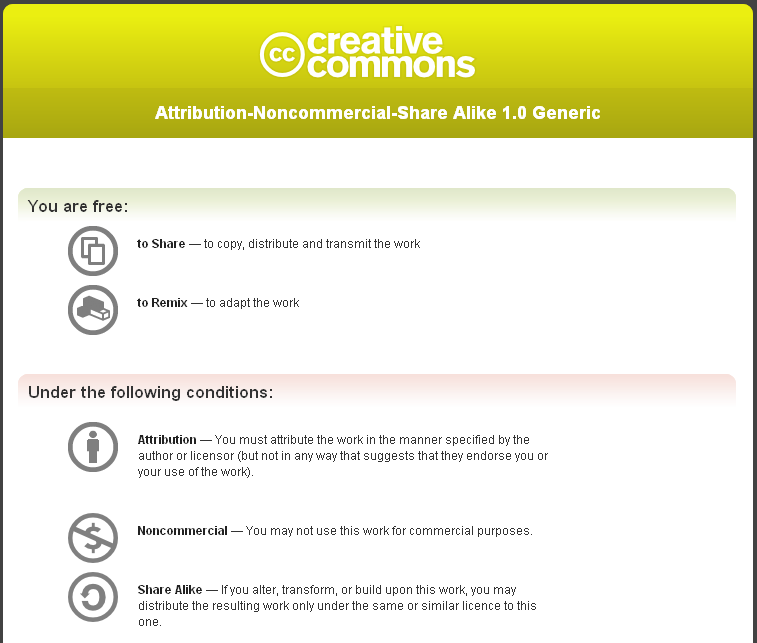
\includegraphics[width=0.74\textwidth]
	{pics/creative_commons.png}
	\caption{\license}
	\label{fig:lisensi}
\end{figure}

Terkait template ini, \pic~\ref{fig:lisensi} diambil dari \url{http://creativecommons.org/licenses/by-nc-sa/1.0/deed.en_CA}. Jika ingin mengentahui lebih lengkap mengenai \license, silahkan buka \url{http://creativecommons.org/licenses/by-nc-sa/1.0/legalcode}.
Seluruh dokumen yang dibuat dengan menggunakan template ini sepenuhnya menjadi hak milik pembuat dokumen dan bebas didistribusikan sesuai dengan keperluan masing-masing.
Lisensi hanya berlaku jika ada orang yang membuat template baru dengan menggunakan template ini sebagai dasarnya.

Penyusun template ingin berterima kasih kepada Andreas Febrian, Lia Sadita, Fahrurrozi Rahman, Andre Tampubolon, dan Erik Dominikus atas kontribusinya dalam template yang menjadi pendahulu template ini.
Penyusun template juga ingin mengucapkan terima kasih kepada Azhar Kurnia atas kontribusinya dalam template yang menjadi pendahulu template ini.

Semoga template ini dapat membantu orang-orang yang ingin mencoba menggunakan \latex.
Semoga template ini juga tidak berhenti disini dengan ada kontribusi dari para penggunanya.
Jika Anda memiliki perubahan yang dirasa penting untuk disertakan dalam template, silakan lakukan \f{fork} repositori Git template ini di \url{https://gitlab.com/ichlaffterlalu/latex-skripsi-ui-2017}, lalu lakukan \f{merge request} perubahan Anda terhadap \f{branch} \code{master}.
Kami berharap agar \f{template} ini dapat terus diperbarui mengikuti perubahan ketentuan dari pihak Rektorat Universitas Indonesia, dan hal itu tidak mungkin terjadi tanpa kontribusi dari teman-teman sekalian.

\vspace*{0.1cm}
\begin{flushright}
Depok, \tanggalSiapSidang\\[0.1cm]
\vspace*{1cm}
\penulis

\end{flushright}
